\section{Implementation Details}
\label{sec:ext}

The implementation follows the client-server model, distributing
measurements of program configurations between a group of virtual
machines running \emph{MeasurementServer}s in the GCE. The servers
waits for measurement requests from a client, and maintain copies
of the program to be autotuned and the user-defined function that
measures configurations.

An interface was also implemented to encapsulate the communication
from the client enabling a considerably lower implementation
effort for the client. Figure~\ref{fig:loc-comp} show a rough
estimate of the implementation effort for the three components
of the implementation.

The machine running the OpenTuner autotuner runs a \emph{MeasurementClient},
an extension of the native \emph{MeasurementDriver}, that instead of
compiling and running result requests locally, uses the GCE interface to
route requests to virtual machines and them saves the results to the local
database.

\begin{figure}[htpb]
    \centering
    \begin{minipage}{.45\textwidth}
        \centering
        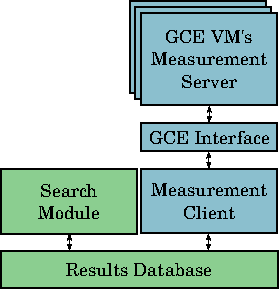
\includegraphics[scale=.64]{high-level-implementation}
        \caption{A high-level view of the architecture.}
        \label{fig:high-level}
    \end{minipage}%
    \hfill
    \begin{minipage}{.45\textwidth}
        \centering
        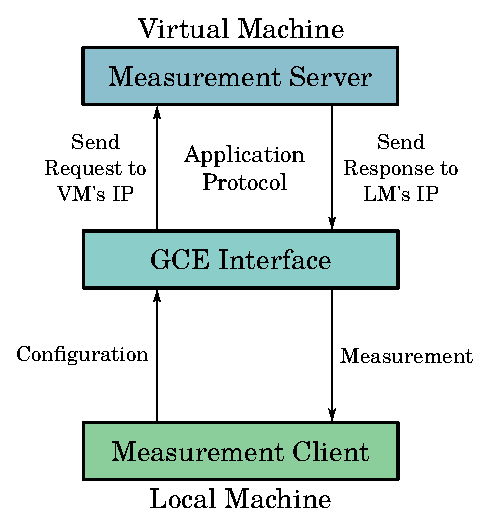
\includegraphics[scale=.64]{low-level-implementation}
        \caption{A lower-level view of the architecture.}
        \label{fig:low-level}
    \end{minipage}%
    \label{fig:archs}
\end{figure}

Figures~\ref{fig:high-level} and~\ref{fig:low-level} present an
overview of the architecture of the extension.
Figure~\ref{fig:high-level} presents the architecture of an OpenTuner
application running the measurement client and communicating with the
measurement servers.  Green boxes in the figure represent OpenTuner modules
that will not be modified, and blue boxes represent new or modified modules.

Figure~\ref{fig:low-level} shows, on a lower level of abstraction, the
interactions between the measurement client and servers. The client
requests results from the server through a wrapper of the GCE Python API.
The GCE interface also encapsulates the application protocol used in
the client-server communication.

The remaining of this section describes the extension implementation in further
detail, the GCE interface and the application protocol.

\begin{figure}[htpb]
    \centering
    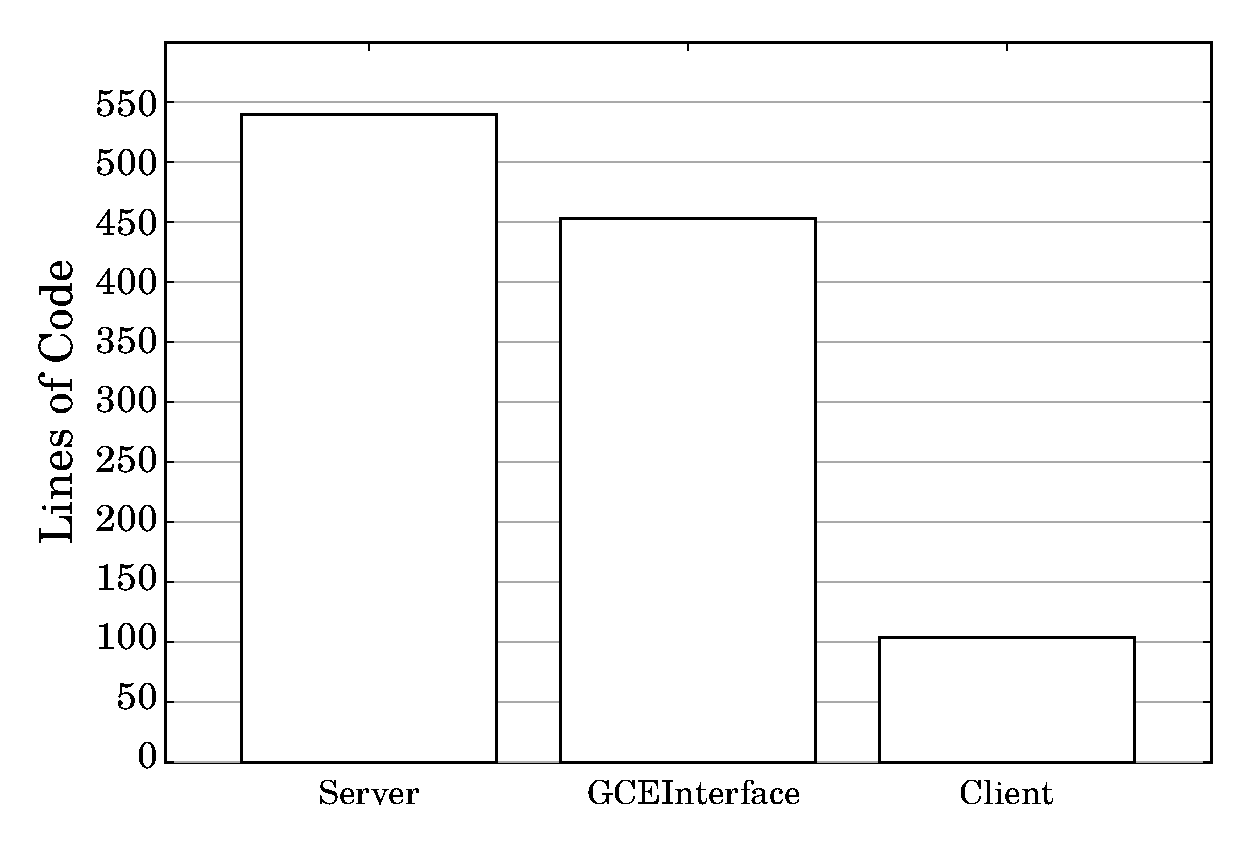
\includegraphics[scale=.35]{loc_comparison}
    \caption{An estimate of the implementation effort, measured in lines of code.}
    \label{fig:loc-comp}
\end{figure}

\subsection{Measurement Server and Client}
\label{sec:server-client}

OpenTuner controls the execution flow of an application with the
\texttt{\footnotesize main} function of the \emph{TuningRunMain} class. This
function initialises the database and the search and measurement modules. It
then calls the \texttt{\footnotesize main} function of the search driver, which
runs the main loop of the application.  The search driver generates
configurations to be tested and saves them to the database. It then calls the
\texttt{\footnotesize process\_all} function of the measurement driver and
blocks until the function returns.

The \texttt{\footnotesize process\_all} function calls the
\texttt{\footnotesize run\_desired\_results} function, which is able to run
compilations in parallel but only sequential measurements.  The modified
\emph{MeasurementDriver} initialises the GCE interface during its own
initialisation. During execution the overridden \texttt{\footnotesize
process\_all} and \texttt{\footnotesize run\_desired\_results} functions route
the result requests to the virtual machines using the \emph{GCEInterface}.

An instance of the \emph{MeasurementServer} runs in every virtual machine. The
server is installed after the machine's initialisation and waits for TCP
connections from a single client. The application protocol used in
communications between the clients and servers is described in
Section~\ref{sec:app}.

\subsection{GCE Interface}
\label{sec:gce}

The interactions between the local \emph{MeasurementClient} and the virtual
machines' \emph{MeasurementServer}s are mediated by the
\emph{GCEInterface}, a wrapper of the GCE Python API.
The interface starts and configures virtual machines
storing each measurement server's IP.

The interface enables the \emph{MeasurementClient} to request results from
the servers without knowledge of the application protocol. Running our
client-server implementation in another cloud environment would require a
new interface that manages virtual machines in this environment, but no
modifications are needed to the server or client.

\subsection{Application Protocol}
\label{sec:app}

This section describes the text-based application protocol used in the
client-server communications mediated by the \emph{GCEInterface}. Note the
\texttt{\footnotesize CLONE} message. The user's OpenTuner application must
be a git project available via \texttt{\footnotesize{HTTP}}. The application
will be cloned to the virtual machine by the server and used to obtain the
autotuning results requested by the client.

\paragraph{Messages}
\newcolumntype{K}{>{\centering\arraybackslash}m{5cm}}
\newcommand{\specialcell}[2][c]{%
  \begin{tabular}[#1]{@{}K@{}}#2\end{tabular}}

\newcolumntype{T}{>{\centering\arraybackslash}m{1.5cm}}
\newcolumntype{L}{>{\centering\arraybackslash}m{2.4cm}}

\begin{table}[htpb]
    \centering
    \tiny
    \begin{tabular}{@{}TLK@{}}
        \toprule
        {\bf Command} & {\bf Function} & {\bf Message} \\ \midrule
        {\tiny \bf START} & 
        {\tiny Sets the server's status to AVAILABLE} & 
        {\tiny \tt ``START''} \\ \midrule
        {\tiny \bf STOP} & 
        {\tiny Sets the server's status to STOPPED} & 
        {\tiny \tt ``STOP''} \\ \midrule
        {\tiny \bf STATUS} & 
        {\tiny Requests the server current status} & 
        {\tiny \tt ``STATUS''} \\ \midrule
        {\tiny \bf DISCONNECT} & 
        {\tiny Disconnects from the server} & 
        {\tiny \tt ``DISCONNECT''} \\ \midrule
        {\tiny \bf SHUTDOWN} & 
        {\tiny Disconnects and shuts the server down} & 
        {\tiny \tt ``SHUTDOWN''} \\ \midrule
        {\tiny \bf CLONE} & 
        {\tiny Clones a git repository to the virtual machine} & 
        {\tiny \tt ``CLONE REPO\_URL DIST\_DIR''} \\ \midrule
        {\tiny \bf LOAD} & 
        {\tiny Imports the user's MeasurementInterface into the server} & 
        {\tiny \tt ``LOAD TUNER\_PATH INTERFACE\_NAME''} \\ \midrule
        {\tiny \bf MEASURE} & 
        {\tiny Computes the measurement for a given configuration} & 
        {\tiny \tt ``MEASURE CONFIG INPUT LIMIT''} \\ \midrule
        {\tiny \bf GET} & 
        {\tiny Requests a configuration's result} & 
        {\tiny \tt ``GET RESULT\_ID''} \\ \bottomrule
    \end{tabular}
    \caption{Server messages.}
    \label{tab:protocol-messages}
\end{table}


Table~\ref{tab:protocol-messages} shows all the messages in the protocol,
a brief description of their meaning and their string format. The client
must send a \texttt{\footnotesize MEASURE} message for each configuration
that is measured. The server returns a unique ID that is used to retrieve
the results when they are ready. This is done by sending a
\texttt{\footnotesize GET} message.

\paragraph{Server Responses}

The server responds to each request with a message template and
trailing, message-specific parameters. Responses always start
with the correspondent command name and end with a newline character.
Each response contains the current server status (\texttt{\footnotesize SERVER\_STATUS})
and error code of the command (\texttt{\footnotesize ERROR\_STATUS}).
The optional argument list (\texttt{\footnotesize [ARGS..]}) contains the
measurement result, for example, in the case of a successful
\texttt{\footnotesize GET} response. Figure~\ref{fig:response-template}
shows the format of a server response.

\begin{figure}[htpb]
    \centering
    \footnotesize
    \begin{tabular}{@{}c@{}}
        \toprule
        {\tt \lq{}COMMAND ERROR\_STATUS SERVER\_STATUS [ARGS..] [MESSAGE]\rq{}} \\ \bottomrule
    \end{tabular}
    \caption{The format of a server response.}
    \label{fig:response-template}
\end{figure}

\paragraph{Code Availability}

The code for the measurement server, client and the interface is
available\footnote{All code is hosted at GitHub: \\ \texttt{\scriptsize
github.com/phrb/measurement-server} \\ \texttt{\scriptsize
github.com/phrb/gce\_interface} \\ \texttt{\scriptsize
github.com/phrb/measurement\_client}} under the GNU General Public License.
